\documentclass[a4paper,12pt]{article}
\usepackage{amsmath}
\usepackage{tikz}
\usepackage{graphicx}
\usepackage{geometry}
\geometry{margin=1in}
\usepackage{float}
\usepackage{subcaption}
\title{\textbf{Design and Demonstration of a Mod-7 Asynchronous Counter Using T Flip-Flops and Arduino Clock}}
\author{Sai Akhila Reddy Turpu - EE24BTECH11055\\Sai Akshitha Suguru - EE24BTECH11054}
\date{}

\begin{document}

\maketitle

\section*{1. Objective}
To design a \textbf{Mod-7 asynchronous counter} using \textbf{T Flip-Flops} and observe its performance using a \textbf{Cathode Ray Oscilloscope (CRO)} with a clock signal provided by an \textbf{Arduino}.

\section*{2. Introduction}
Counters are sequential digital circuits used for counting pulses. A \textbf{Mod-7 counter} counts from 0 to 6, cycling through 7 distinct states. 

An \textbf{asynchronous counter} (also known as a ripple counter) is one in which the clock is applied only to the first flip-flop, and the output of each flip-flop serves as the clock for the next. The \textbf{T (Toggle) Flip-Flop} is ideal for this purpose as it toggles its state on every active clock edge when the T input is high.

For a Mod-7 counter:
\begin{itemize}
    \item Number of required states = 7
    \item Minimum number of flip-flops = $3$
    \item Number of states with 3 FFs = $2^3 = 8$ (so 1 unused state must be avoided)
\end{itemize}



\section*{3. Truth Table}
The truth table for the Mod-7 counter is as follows:

\begin{center}
\begin{tabular}{|c|c|c|c|}
\hline
Clock Pulse & Q2 (MSB) & Q1 & Q0 (LSB) \\
\hline
0 & 0 & 0 & 0 \\
1 & 0 & 0 & 1 \\
2 & 0 & 1 & 0 \\
3 & 0 & 1 & 1 \\
4 & 1 & 0 & 0 \\
5 & 1 & 0 & 1 \\
6 & 1 & 1 & 0 \\
\hline
\end{tabular}
\end{center}

The state 111 is unused and must be forced to reset to 000.

\begin{table}[H]
    \centering
    \renewcommand{\arraystretch}{1.2}
    \begin{tabular}{|c|c|c|c|c|}
        \hline
        T & Q(n) & J & K & Q(n+1)\\ 
        \hline
        0 & 0 & 0 & X & 0\\ 
        0 & 1 & X & 0 & 1\\ 
        1 & 0 & 1 & X & 1\\ 
        1 & 1 & X & 1 & 0\\ 
        \hline
    \end{tabular}
    \caption{Conversion of JK Flip-Flop to T Flip-Flop}
\end{table}

\section*{4. Circuit Diagram}
\begin{itemize}
    \item Three T Flip-Flops connected in series.
    \item T inputs are held high (T=1) for toggle behavior. Hence we set J and K input to 1.  
    \item Clock is applied to the first JK FF.
    \item Output of one flip-flop is connected as clock to the next (ripple configuration).
    \item A logic gate (NAND) detects the unused state (111) and resets the counter.
\end{itemize}

\begin{figure}[H]
    \centering
    % First image
    \begin{subfigure}[b]{0.45\textwidth}
        \centering
        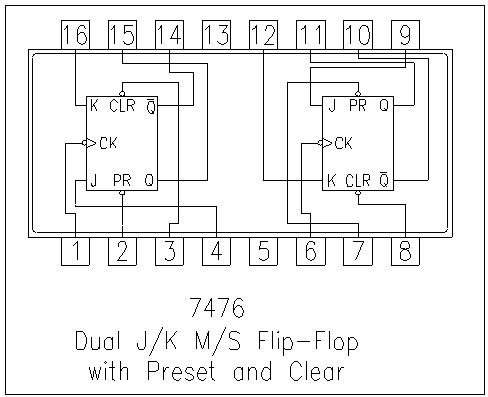
\includegraphics[width=\linewidth]{figs/IC7476.png} % Replace with your image
	    \caption{IC7476 pin diagram}
        \label{fig:image1}
    \end{subfigure}
    \hfill % Adds space between images
    % Second image
    \begin{subfigure}[b]{0.45\textwidth}
        \centering
        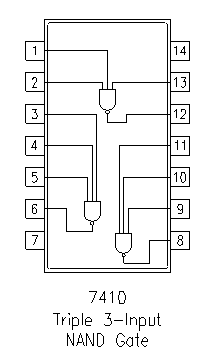
\includegraphics[width=\linewidth]{figs/7410.png} % Replace with your image
        \caption{IC7410 pin diagram}
        \label{fig:image2}
    \end{subfigure}
    
    \caption{Pin diagrams}
    \label{fig:side_by_side}
\end{figure}


\begin{center}
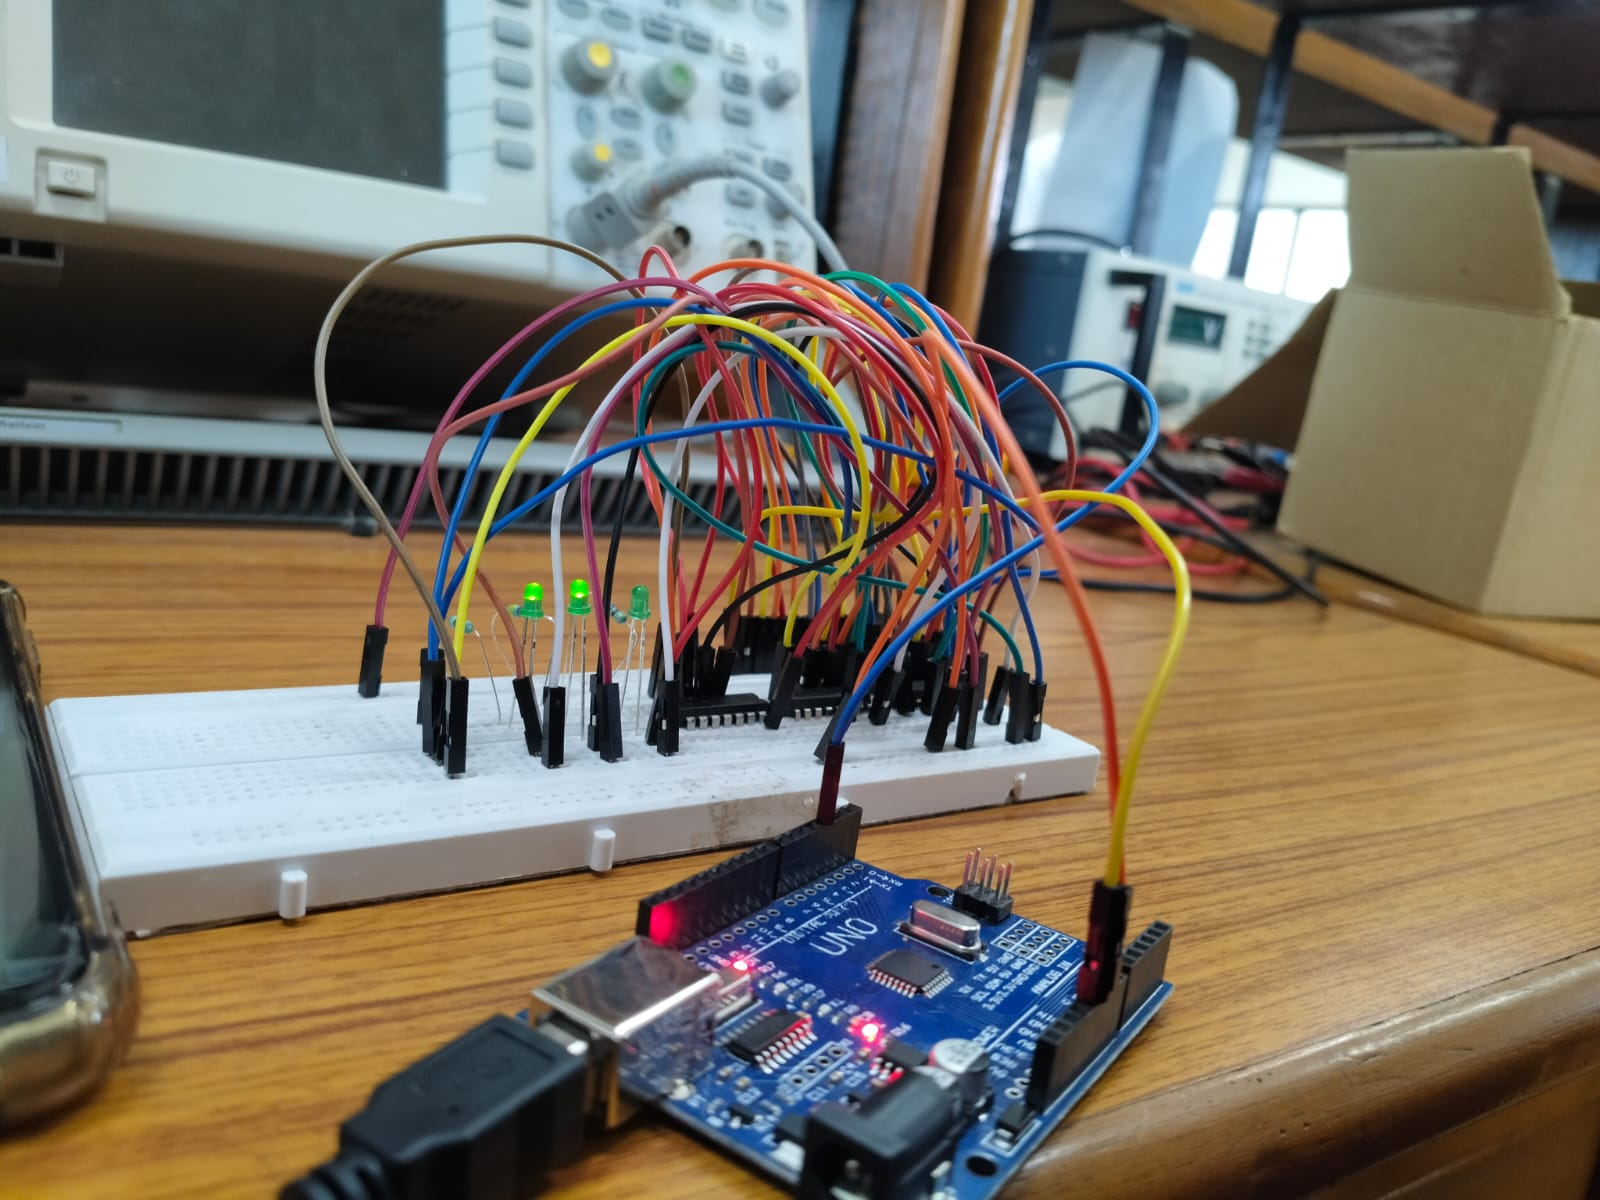
\includegraphics[width=0.8\textwidth]{figs/ckt.jpeg} % Replace with your circuit diagram image
\end{center}



\section*{5. Arduino Clock Generation}
The Arduino can be programmed to generate a square wave clock signal using a digital output pin and delay.

\subsection*{Arduino Code}
\begin{verbatim}
void setup() {
  pinMode(3, OUTPUT);
}
void loop() {
  digitalWrite(3, HIGH);
  delay(1000); // 1000 ms high
  digitalWrite(3, LOW);
  delay(1000); // 1000 ms low
}
\end{verbatim}

\textit{Note: Pin 3 provides a 2 Hz clock pulse (adjust delay for frequency).}

\begin{figure}[H]
    \centering
    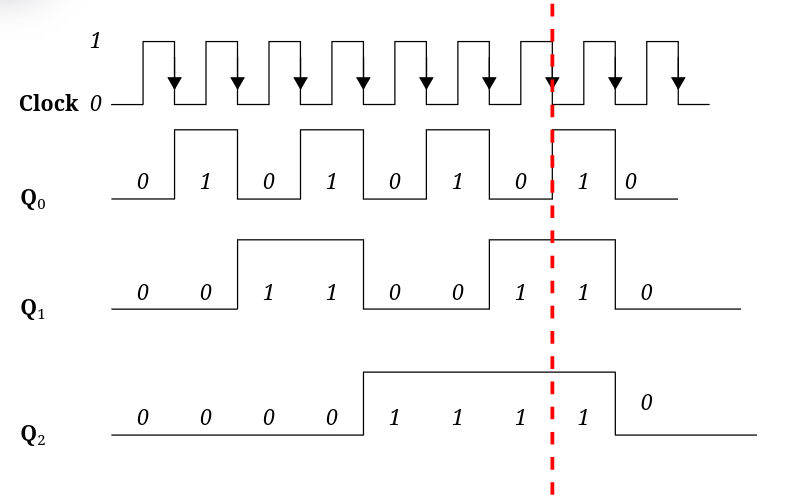
\includegraphics[width=0.6\textwidth]{figs/s.png}  % Replace with your image file
    \caption{Clock signal and output signals of $Q_0$, $Q_1$ and $Q_2$}
    \label{fig:example}
\end{figure}


\section*{6. Observing on CRO}
Connect the Q0, Q1, and Q2 outputs to different channels of the CRO to observe:
\begin{itemize}
    \item Clock signal waveform
    \item Sequential toggling of flip-flop outputs
    \item Reset after the 7th state
\end{itemize}

We see Q0 toggling on every pulse, Q1 toggling every 2 pulses, and Q2 every 4 pulses until reset at state 7.

\begin{figure}[H]
    \centering
    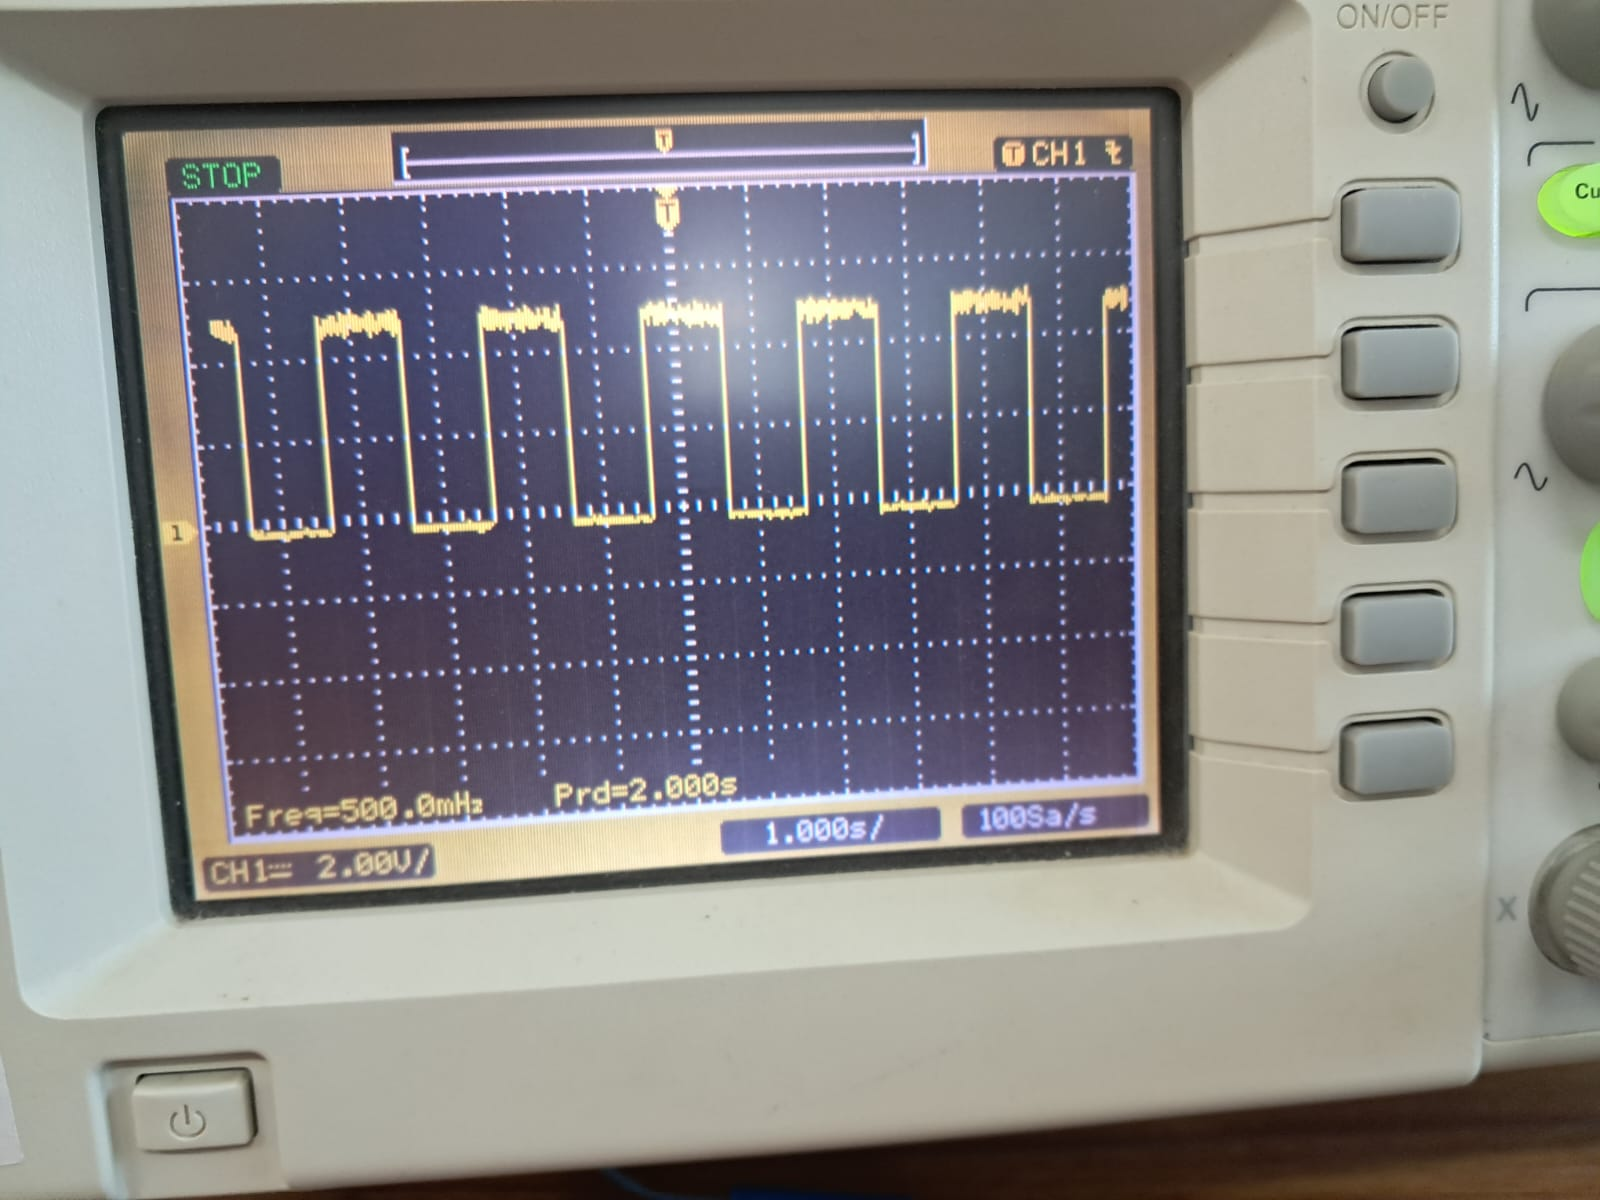
\includegraphics[width=0.6\textwidth]{figs/clock.jpeg} % Update filename
    \caption{Clock Signal: Synchronizes state transitions.}
    \label{fig:clock}
\end{figure}
\textbf{Frequency = 0.5 mHz}
% Figure 2: Q0 Output
\begin{figure}[H]
    \centering
    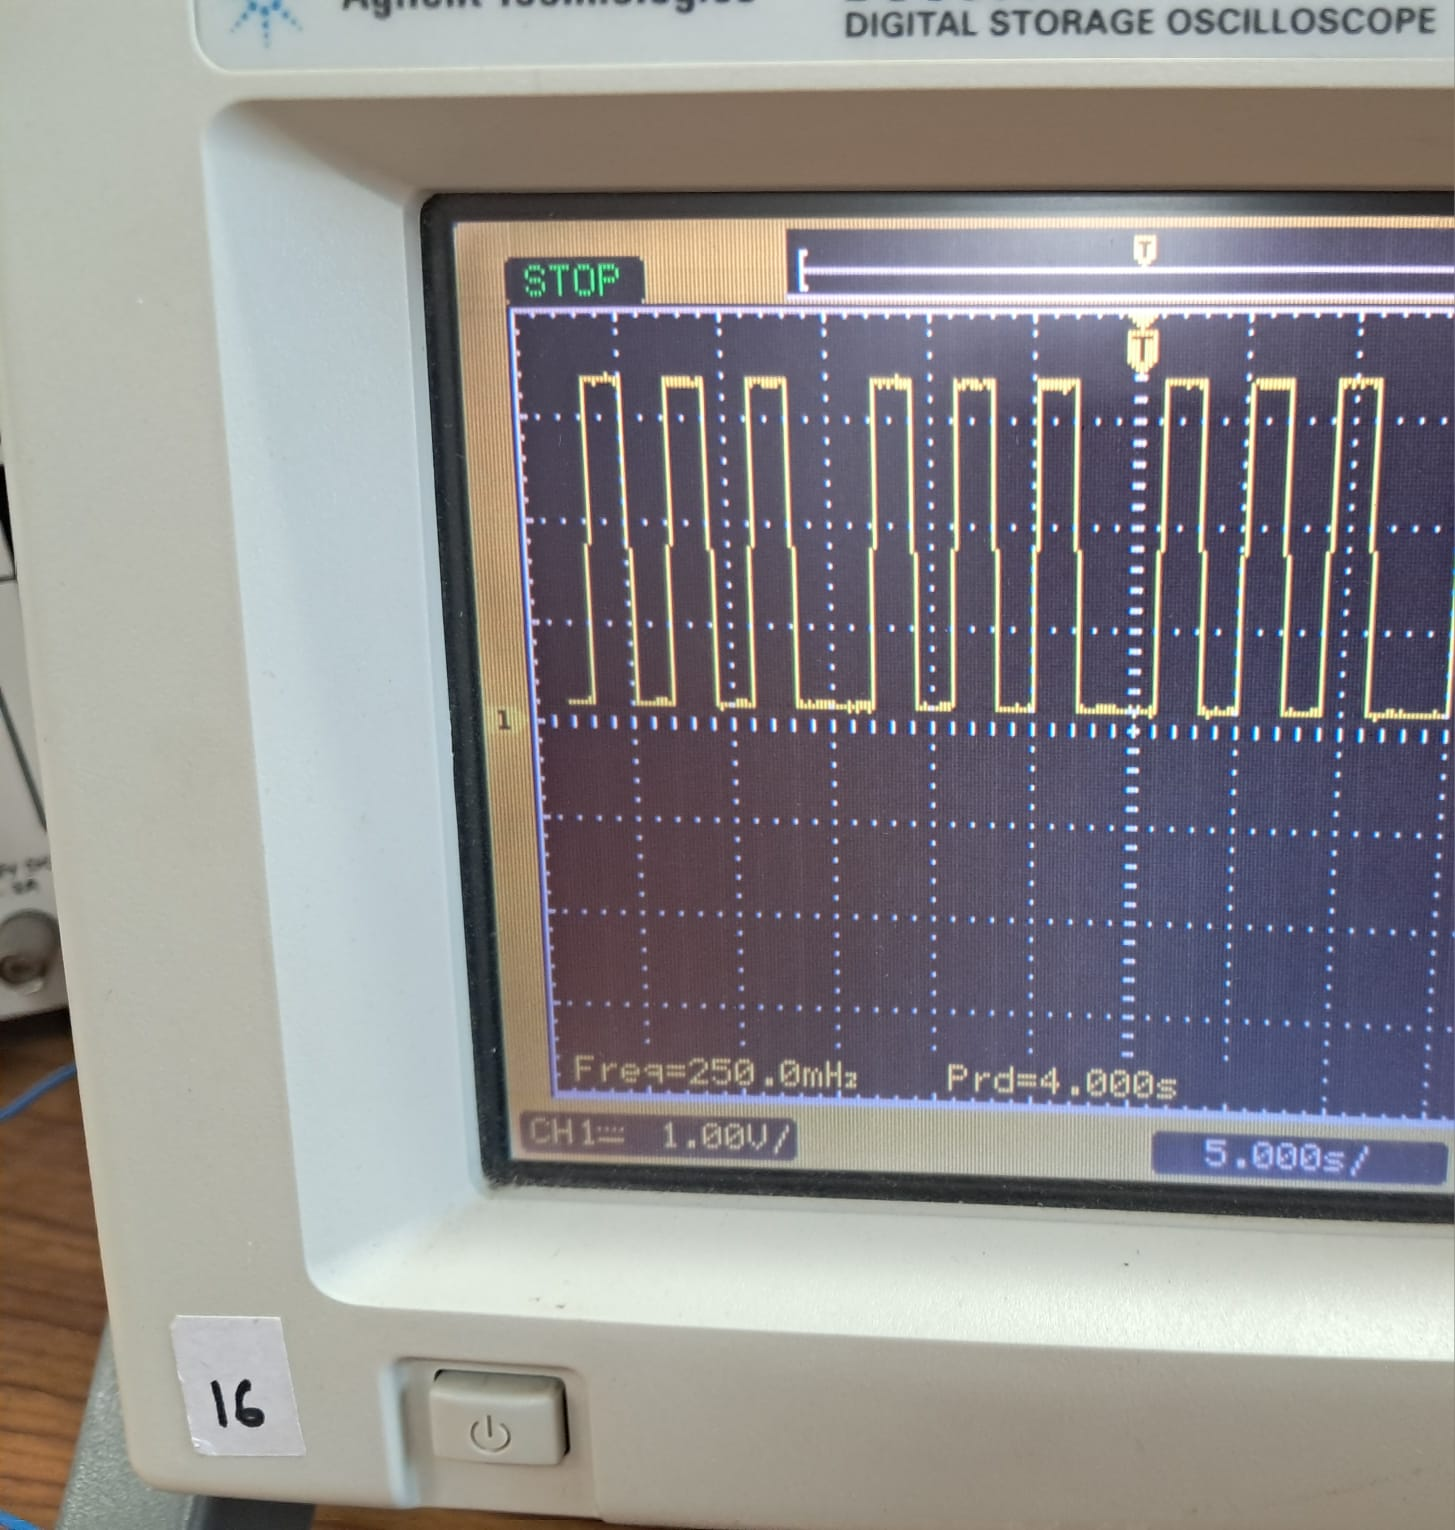
\includegraphics[width=0.6\textwidth]{figs/q0.jpeg} % Update filename
    \caption{Q0 Output: Least significant bit of the counter.}
    \label{fig:q0}
\end{figure}
\textbf{Frequency = f/2 = 0.250 mHz}
% Figure 3: Q1 Output
\begin{figure}[H]
    \centering
    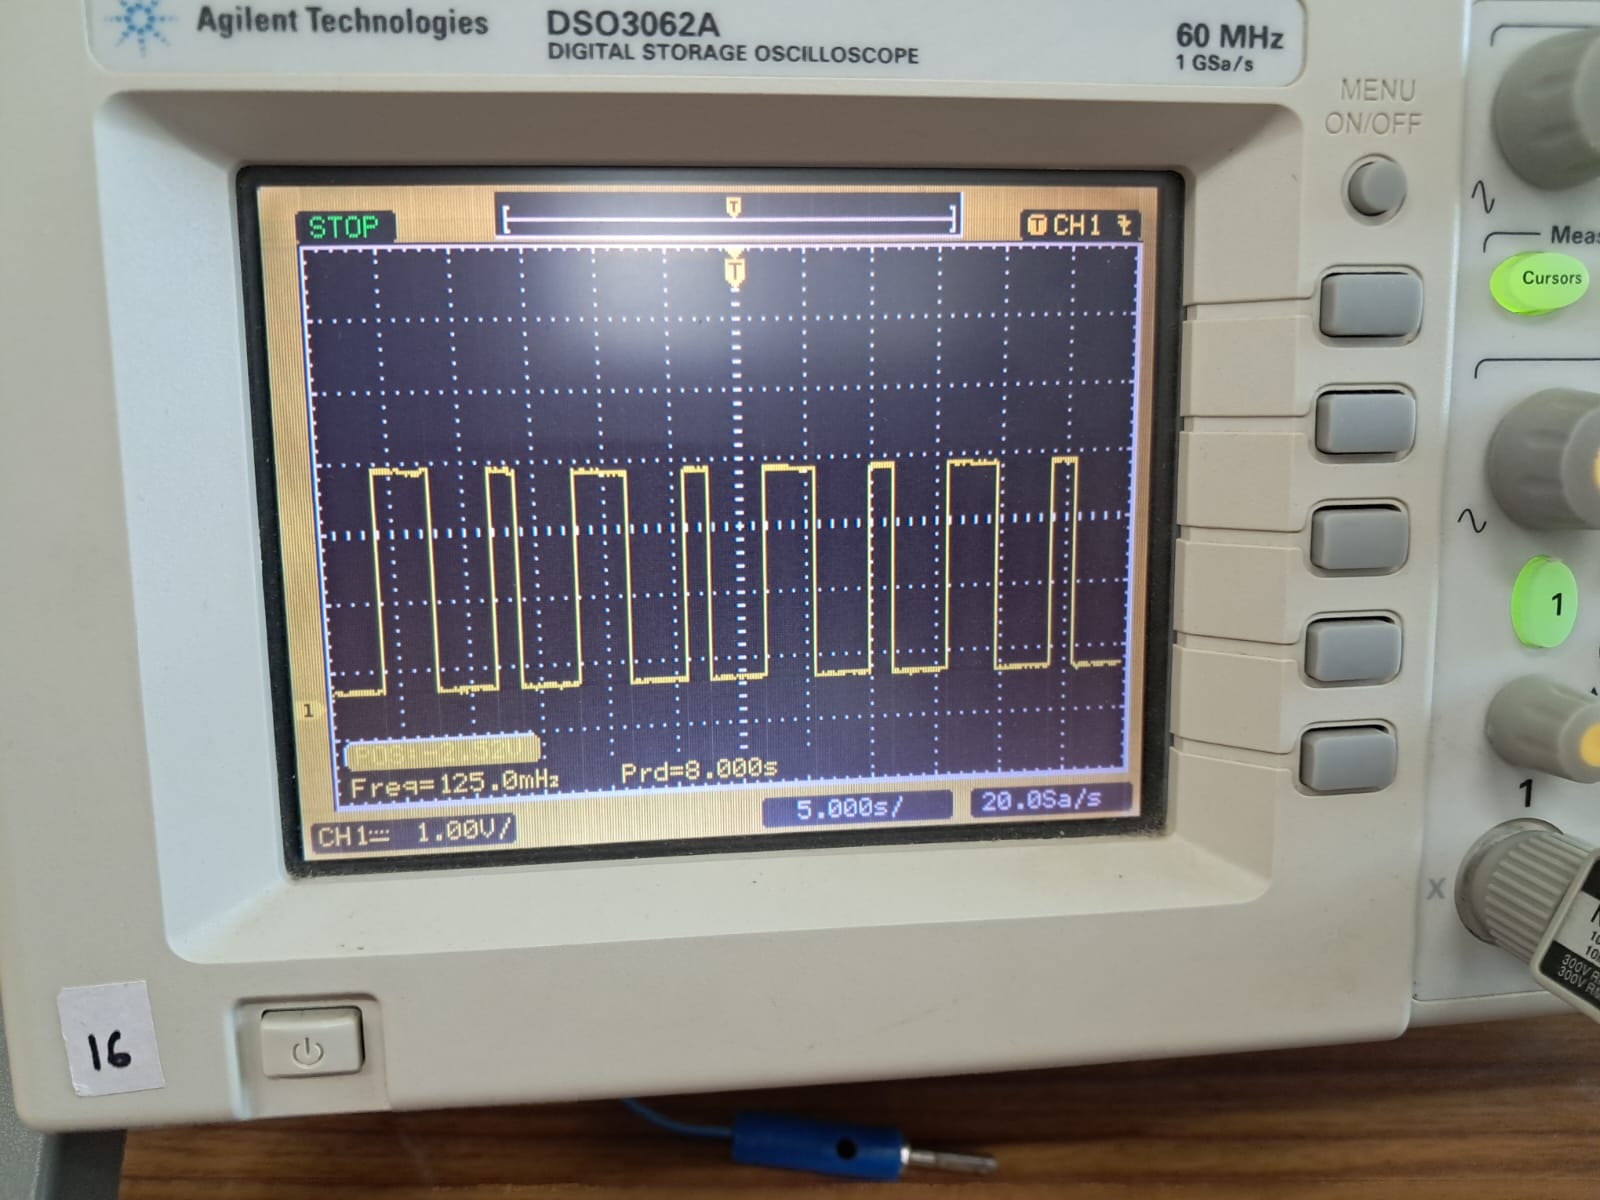
\includegraphics[width=0.6\textwidth]{figs/q1.jpeg} % Update filename
    \caption{Q1 Output: Middle bit of the counter.}
    \label{fig:q1}
\end{figure}
\textbf{Frequency = f/4 = 0.125 mHz}
% Figure 4: Q2 Output
\begin{figure}[H]
    \centering
    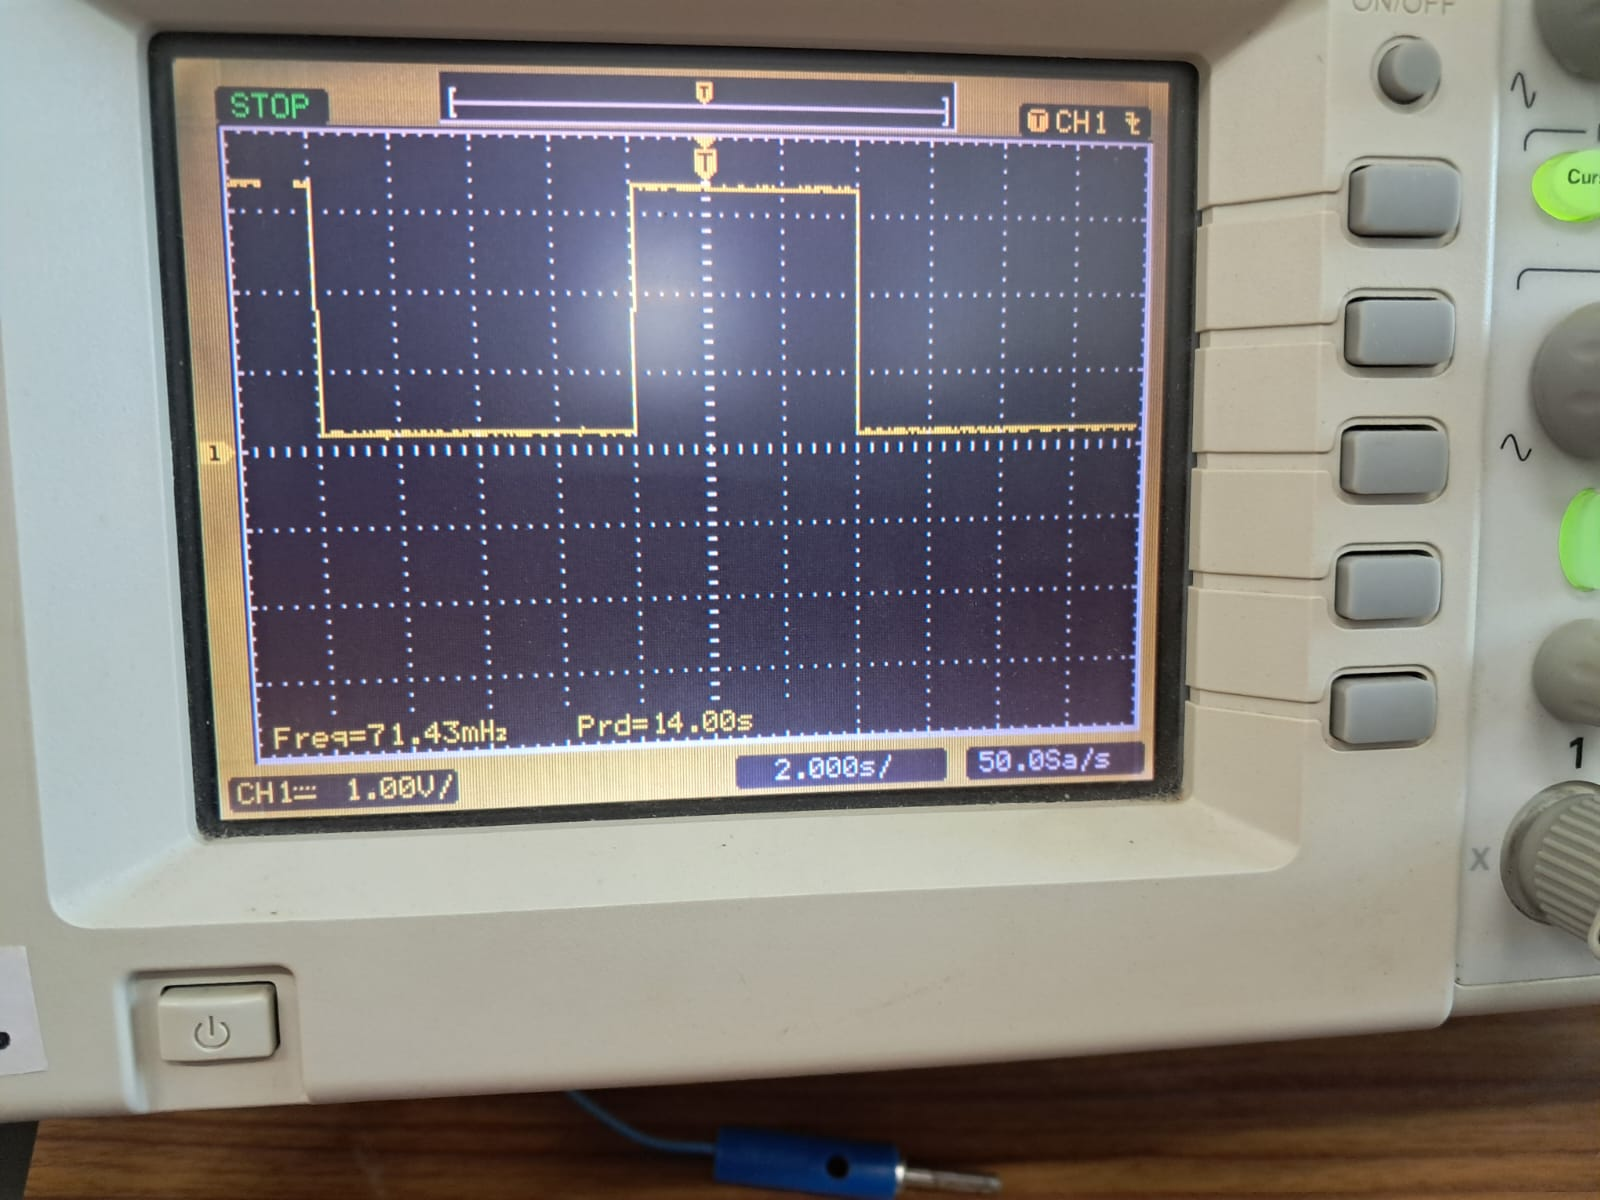
\includegraphics[width=0.6\textwidth]{figs/q2.jpeg} % Update filename
    \caption{Q2 Output: Most significant bit of the counter.}
    \label{fig:q2}
\end{figure}
\textbf{Frequency = 0.7143 mHz}\\
Since 7 is attenuated, the signal which was supposed to be periodic with 16 seconds, now has a new period of 14 seconds. Hence the frequency of the signal is shown as $\frac{1}{14} Hz$ = 0.7143 Hz.

\begin{table}[H]
    \centering
    \begin{tabular}{ccc} % Three columns for images
        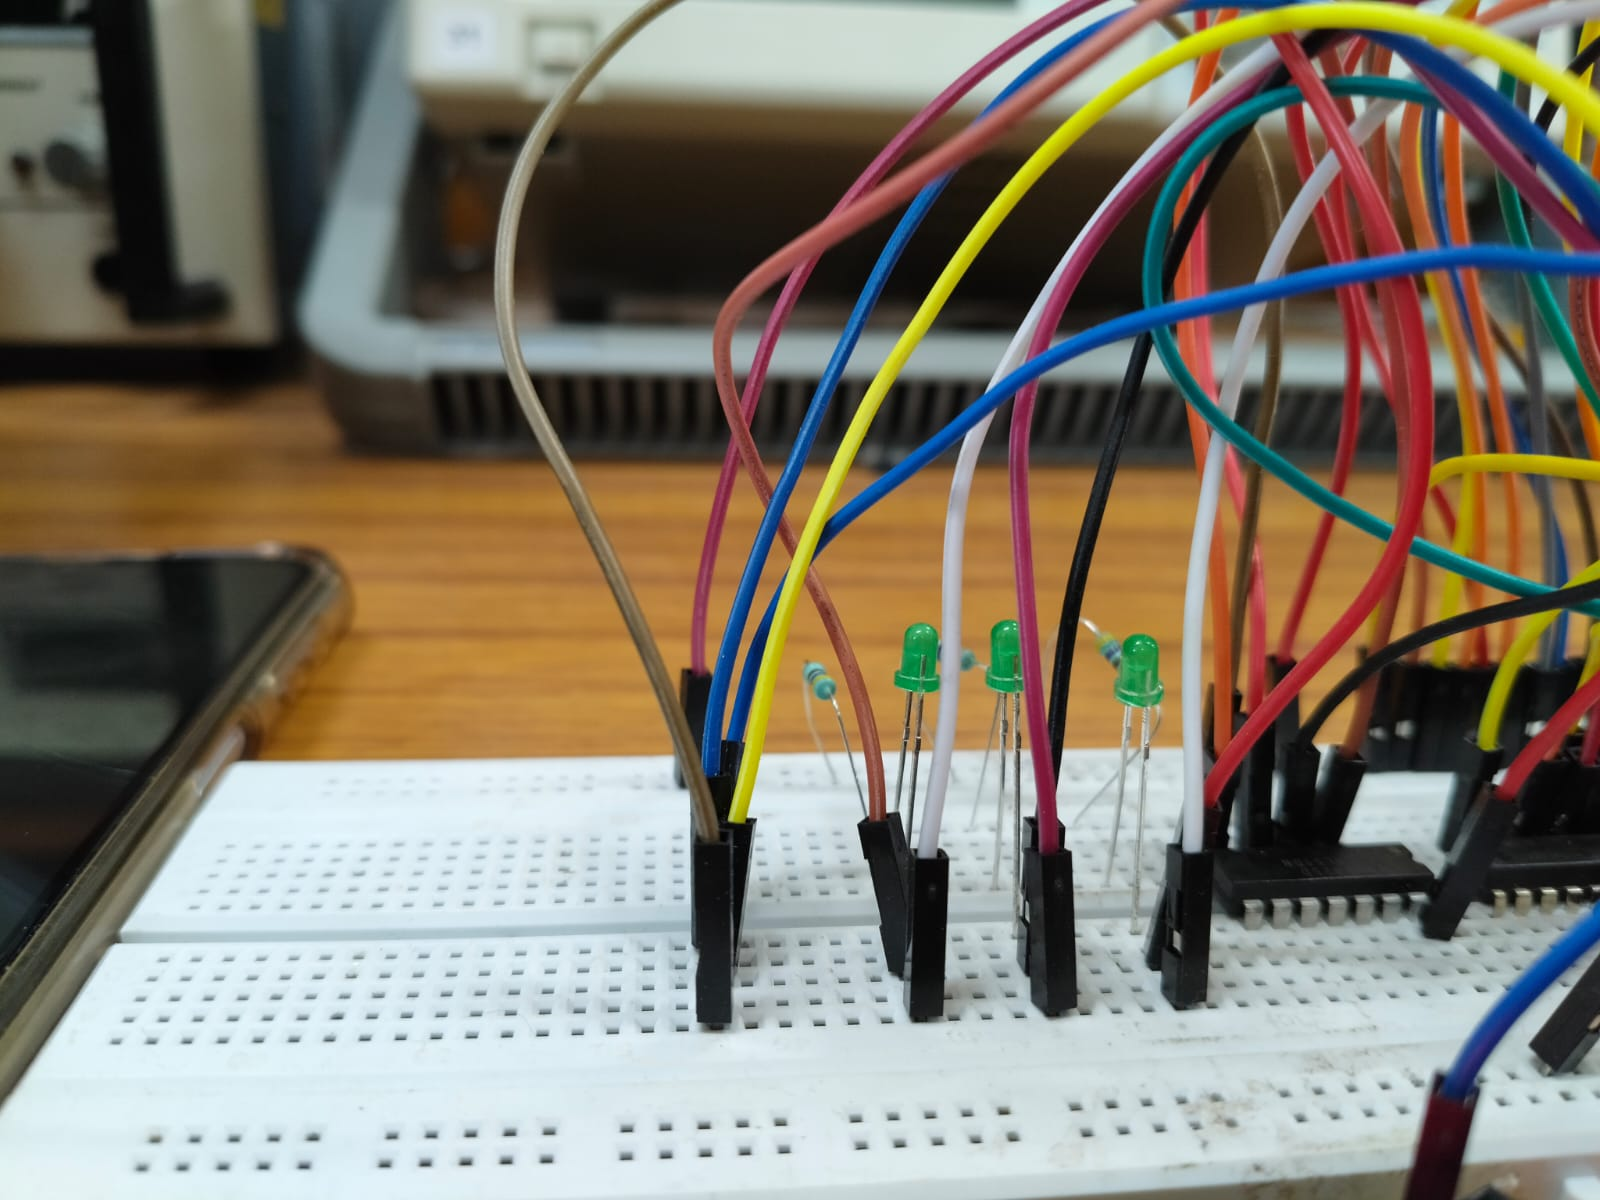
\includegraphics[width=0.3\textwidth]{figs/0.jpeg} & 
        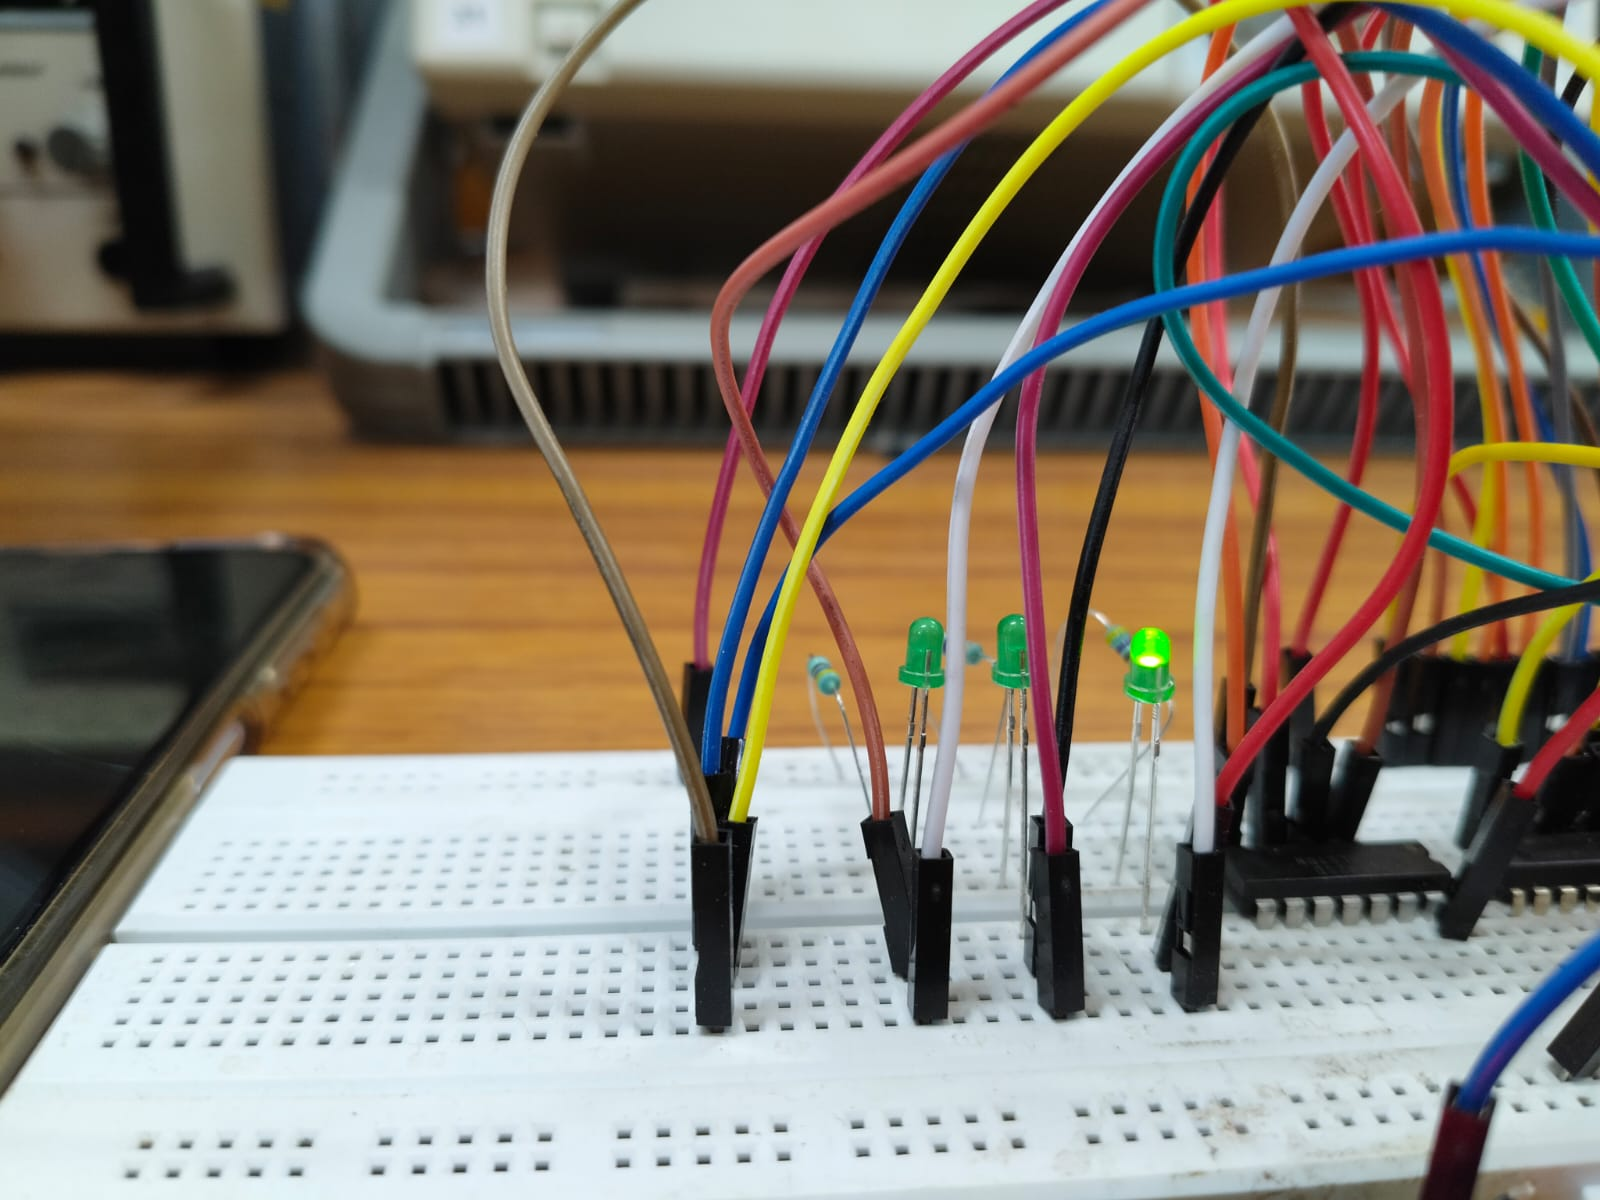
\includegraphics[width=0.3\textwidth]{figs/1.jpeg} & 
        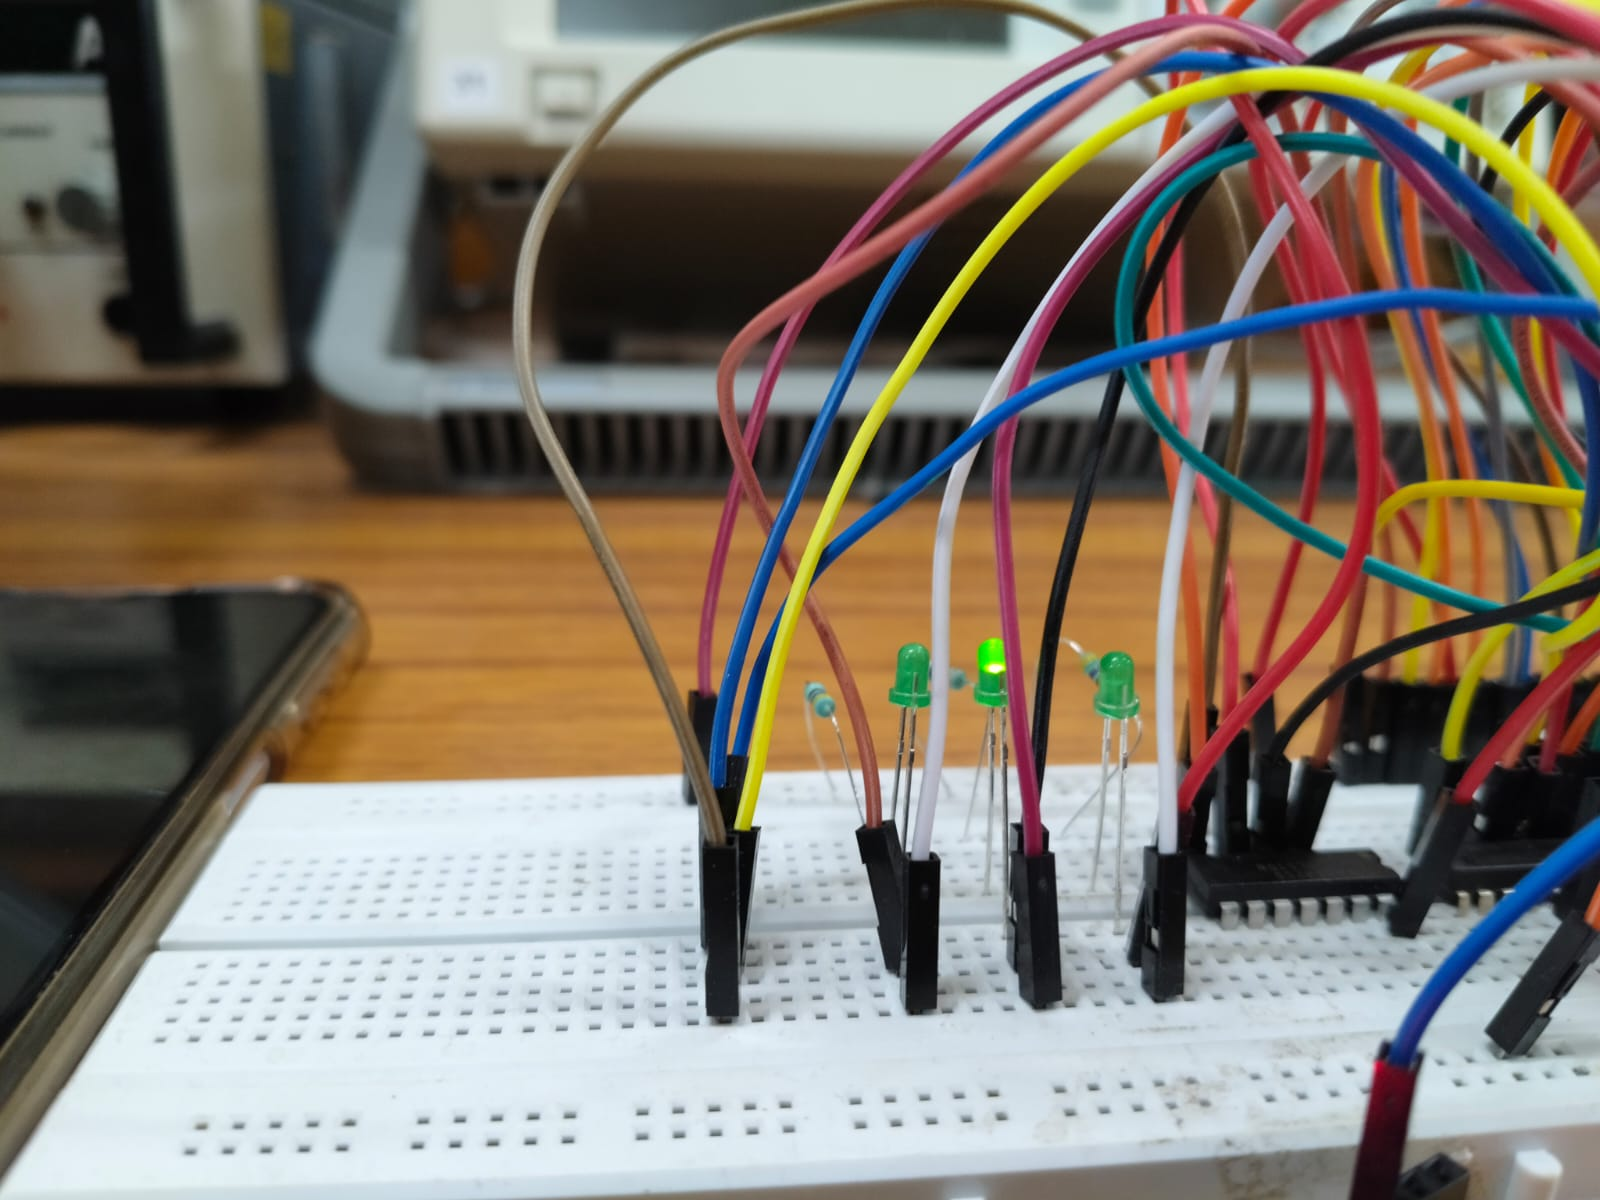
\includegraphics[width=0.3\textwidth]{figs/2.jpeg} \\ 
        Number0 & Number1 & Number2 \\
        
        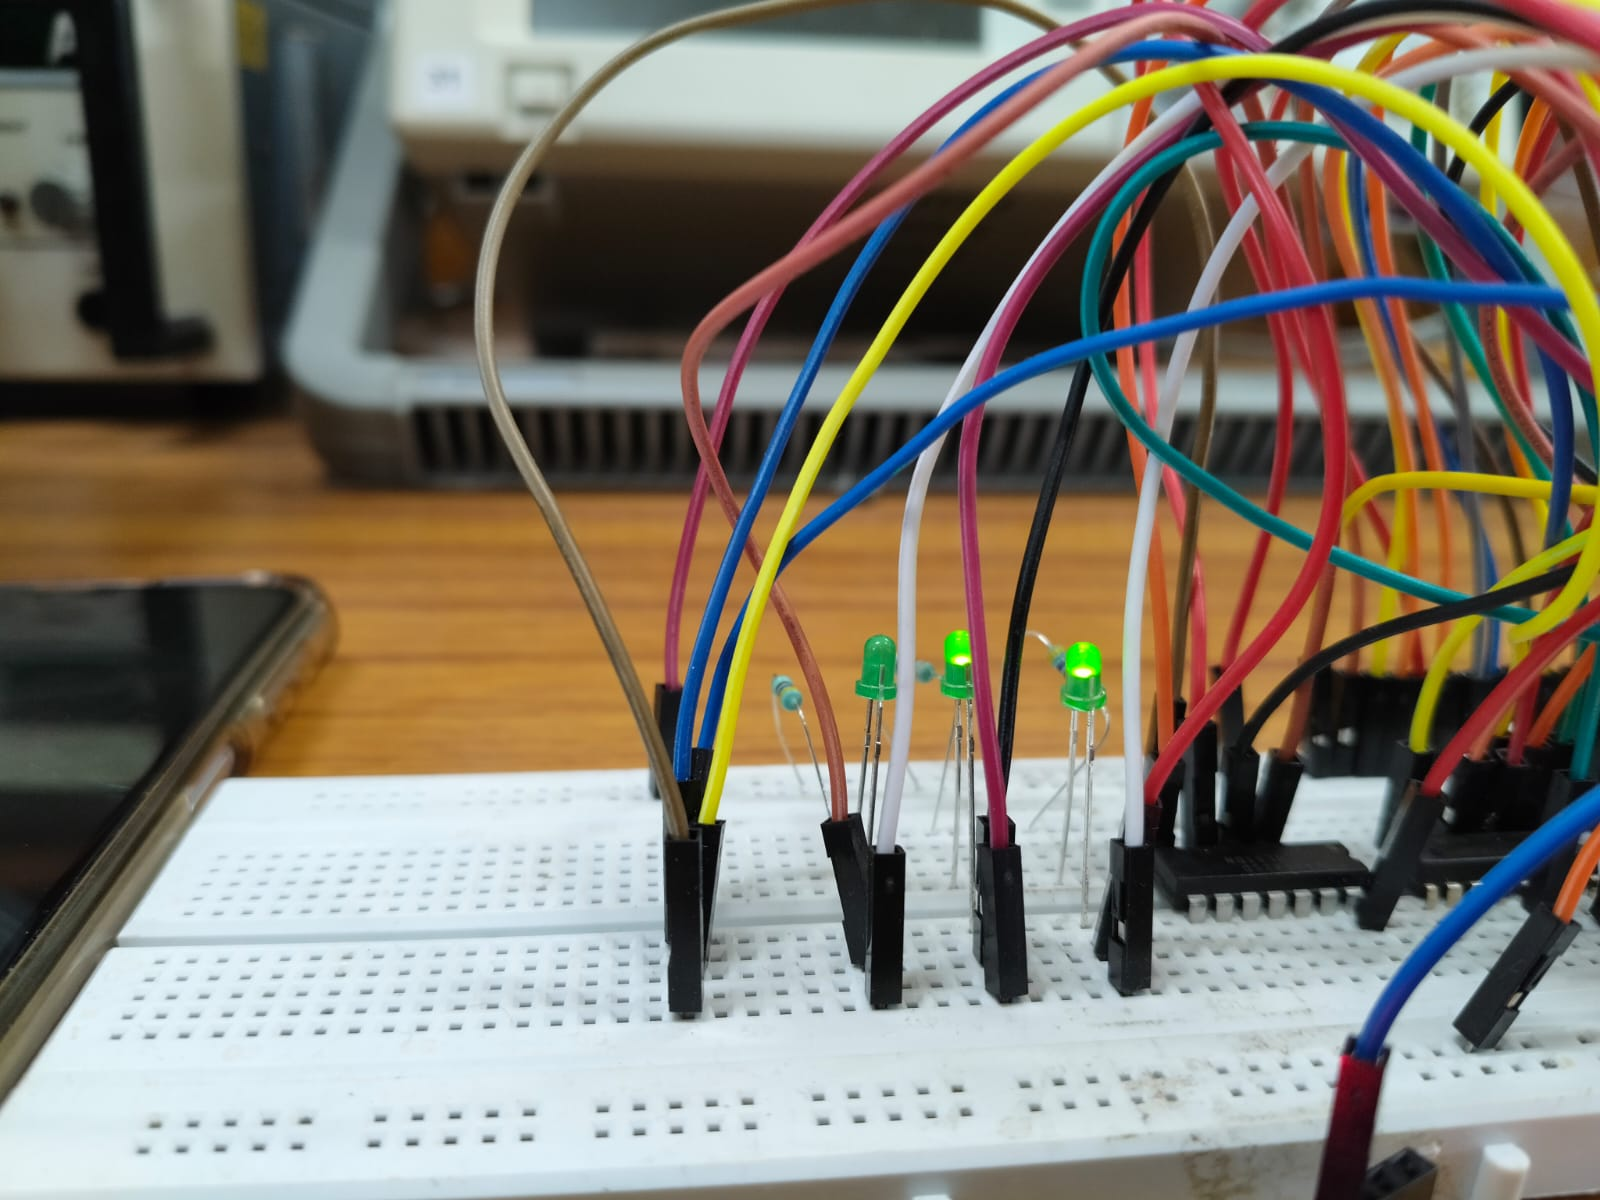
\includegraphics[width=0.3\textwidth]{figs/3.jpeg} & 
        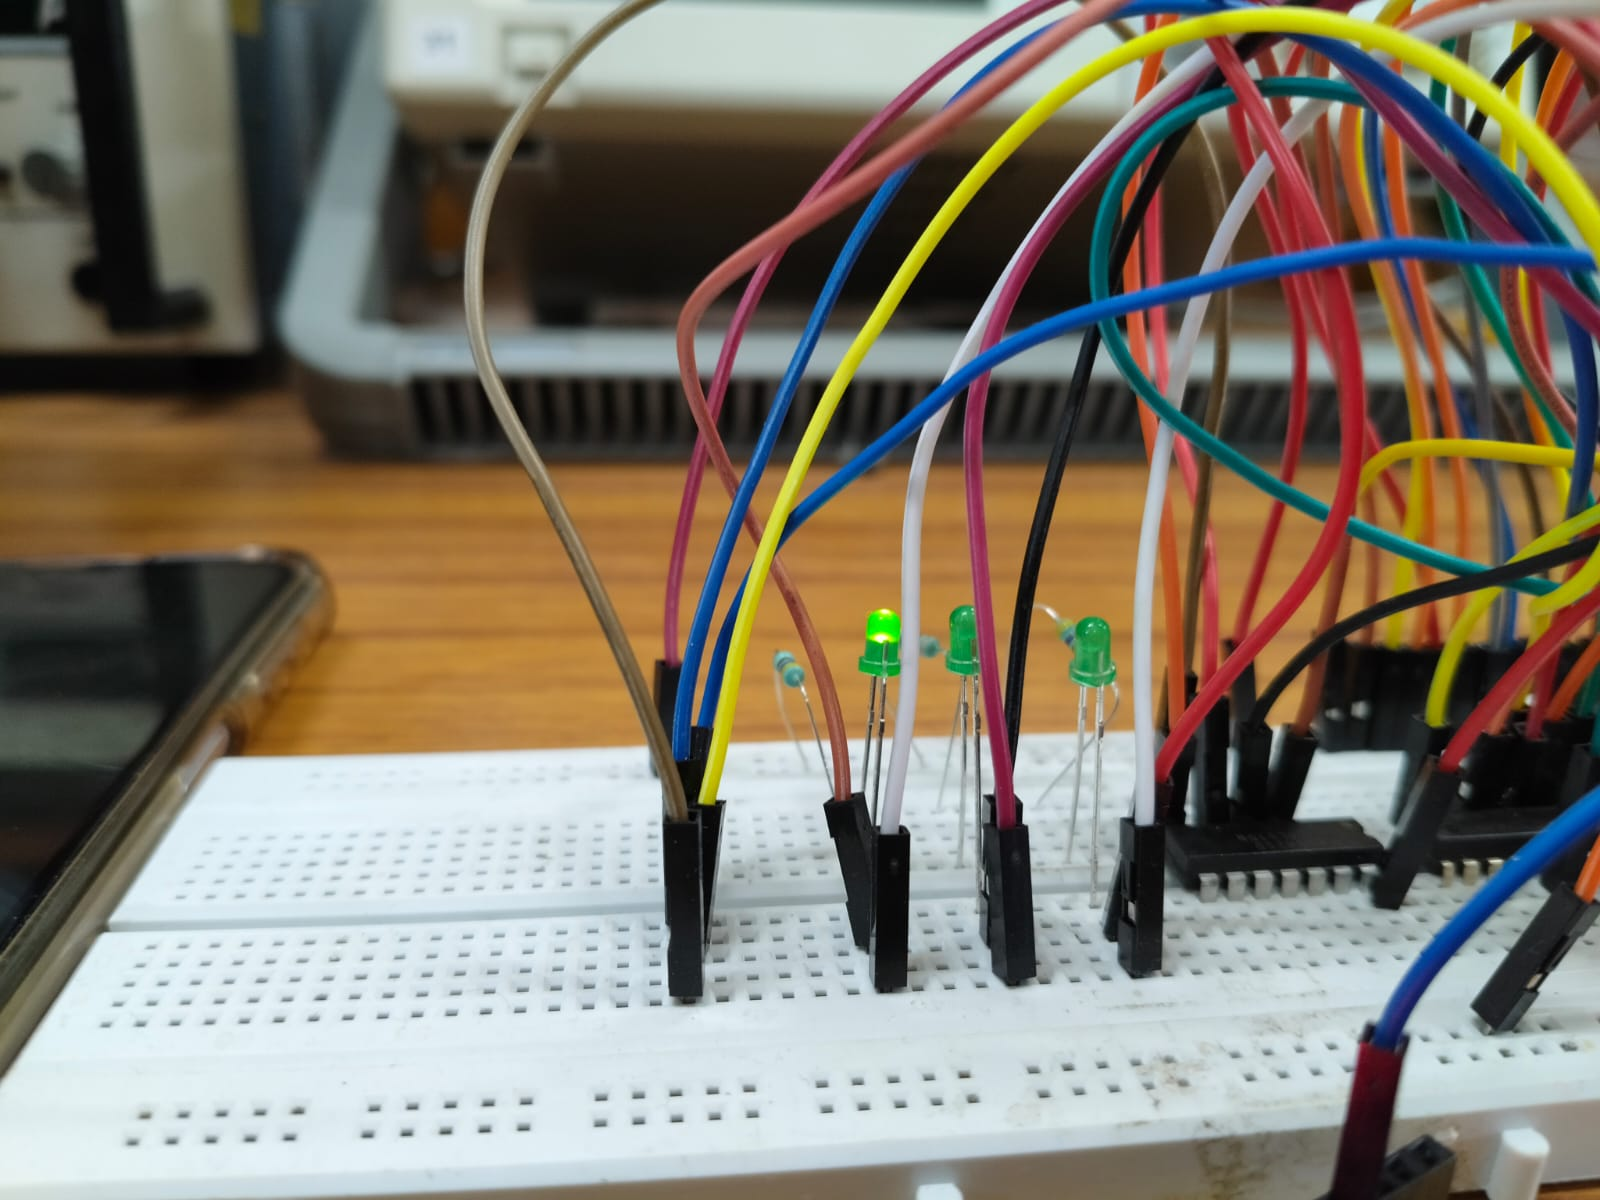
\includegraphics[width=0.3\textwidth]{figs/4.jpeg} & 
        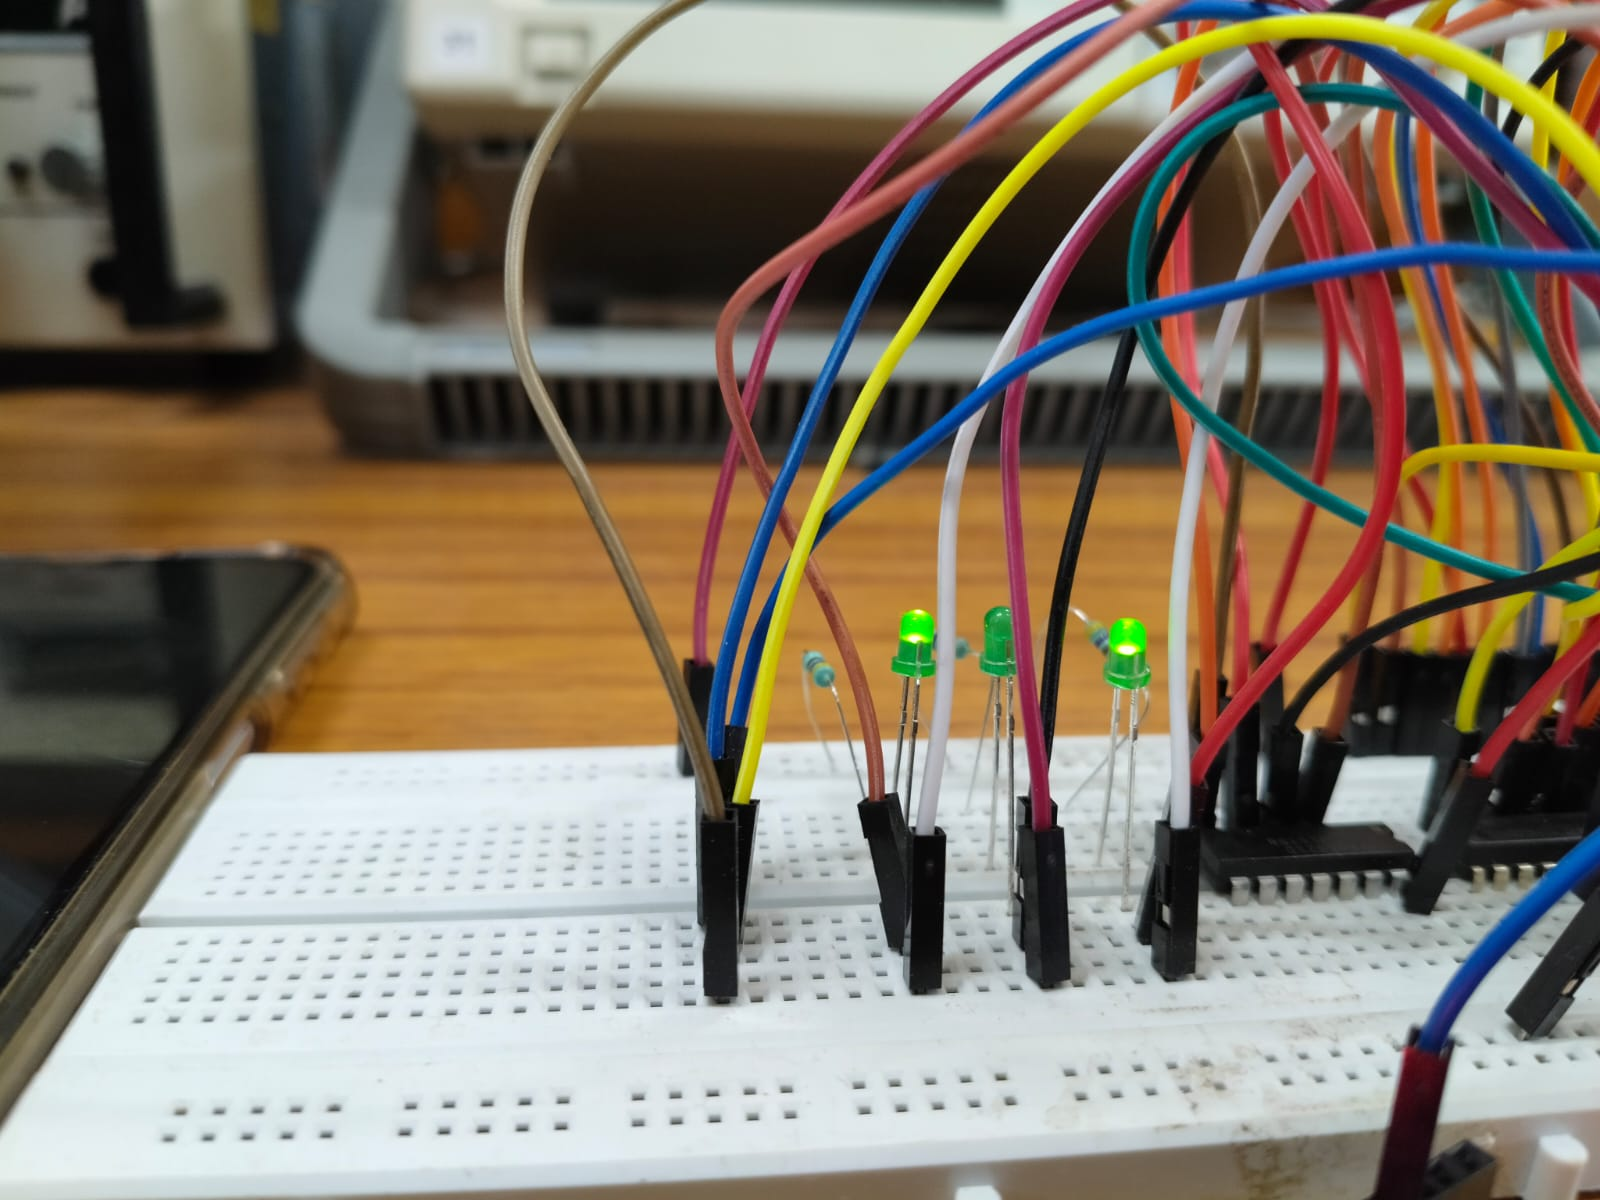
\includegraphics[width=0.3\textwidth]{figs/5.jpeg} \\ 
        Number3 & Number4 & Number5 \\
        
        \multicolumn{3}{c}{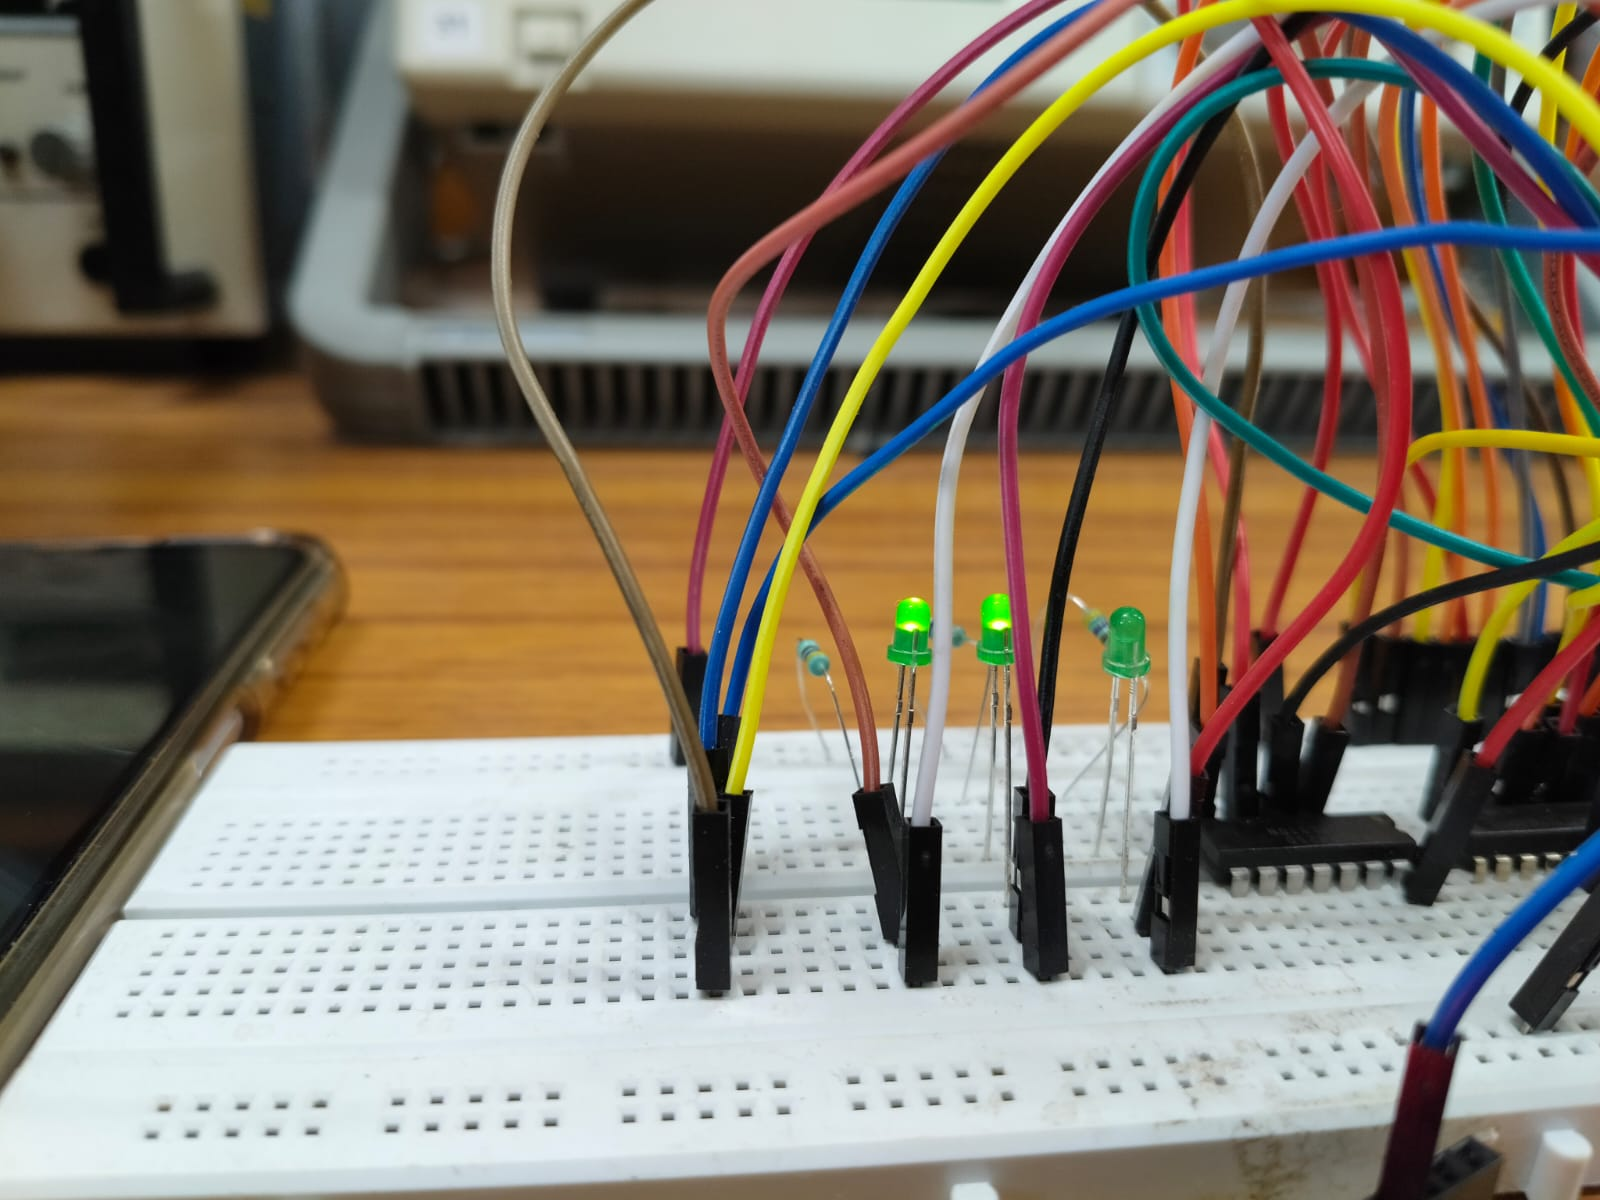
\includegraphics[width=0.3\textwidth]{figs/6.jpeg}} \\
        \multicolumn{3}{c}{Number6}
    \end{tabular}
    \caption{Collection of Number images}
    \label{tab:numbers}
\end{table}

\section*{7. Result}
A working Mod-7 asynchronous counter was successfully designed using T Flip-Flops. Its correct operation was verified using a CRO. The counter counts from 000 to 110 and resets after the 7th pulse. A clock signal from an Arduino was effectively used to drive the circuit.

\section*{8. Conclusion}
This experiment demonstrates the implementation of a Mod-7 asynchronous counter using T flip-flops and illustrates how microcontroller-generated clocks can be used in digital circuits. The counter reliably resets after 7 counts, validating the design logic.



\end{document}

